\documentclass[compress,table,red]{beamer}
\usetheme{Madrid} % Beamer theme v 3.x
\usecolortheme{orchid}
 \usepackage[latin1]{inputenc}
 \usepackage[T1]{fontenc}
 \usepackage[spanish]{babel}

\title{Principio de Sustentaci�n}
\author{Eros Camacho Ruiz}
\begin{document}
	\begin{frame} % Transparencia de presentaci�n
		\titlepage
	\end{frame}
	
		\section{Introducci�n}
	\begin{frame}
		\transboxin
		\frametitle{Introducci�n}
		La {\bf sustentaci�n} es la fuerza generada sobre un cuerpo que se desplaza a trav�s de un fluido, de direcci�n perpendicular a la de la velocidad de la corriente incidente. La aplicaci�n m�s conocida es la del ala , de un ave o un avi�n, superficie generada por un perfil alar.
		
		\pause Como con otras fuerzas aerodin�micas, en la pr�ctica se utilizan coeficientes adimensionales que representan la efectividad de la forma de un cuerpo para producir sustentaci�n y se usan para facilitar los c�lculos y los dise�os.	
	
		\pause El modelo matem�tico de la fuerza de sustentaci�n es:
		
		\begin{equation}
		F_S=\frac{1}{2}{\rho}{V^2}C_L
		\end{equation}
		
		\begin{center}
			\pause	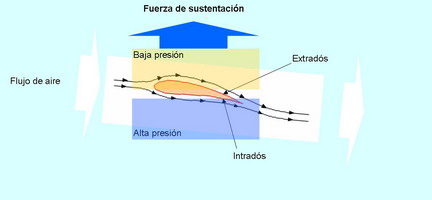
\includegraphics[width=4cm]{principio}	
		\end{center}
		
	\end{frame}
	
	\begin{frame}
		\transboxout
		\frametitle{Introducci�n}
	 	Es la principal fuerza que permite que una aeronave con alas se mantenga en vuelo. �sta, al ser mayor que el peso total de la aeronave, le permite despegar. Tambi�n es muy importante en el automovilismo.
		\pause \par A continuaci�n vamos a ver algunos ejemplos de veh�culos que utilizan este principio para desplazarse:
		\pause \begin{itemize}
			\item VEH�CULOS A�REOS
				\begin{itemize}
					\item F-22 RAPTOR
					\item Eurofighter Typhoon
					\item Airbus A-380
					\item C-130
				\end{itemize}
		\pause	\item VEH�CULOS TERRESTRES
				\begin{itemize}
					\item F�rmula 1
					\item Coches deportivos
				\end{itemize}
		
		\end{itemize}
		
	\end{frame}
	
	\section{Veh�culos a�reos}
	\begin{frame}
		\transblindshorizontal
		\frametitle{Veh�culos a�reos}
		\begin{center}
		\begin{tabular}{m{2.5cm}m{2.5cm}m{2.5cm}m{2.5cm}}
			IMAGEN & AVIONES & PESO (KG) & VEL.MAX(km/h) \\
		\pause	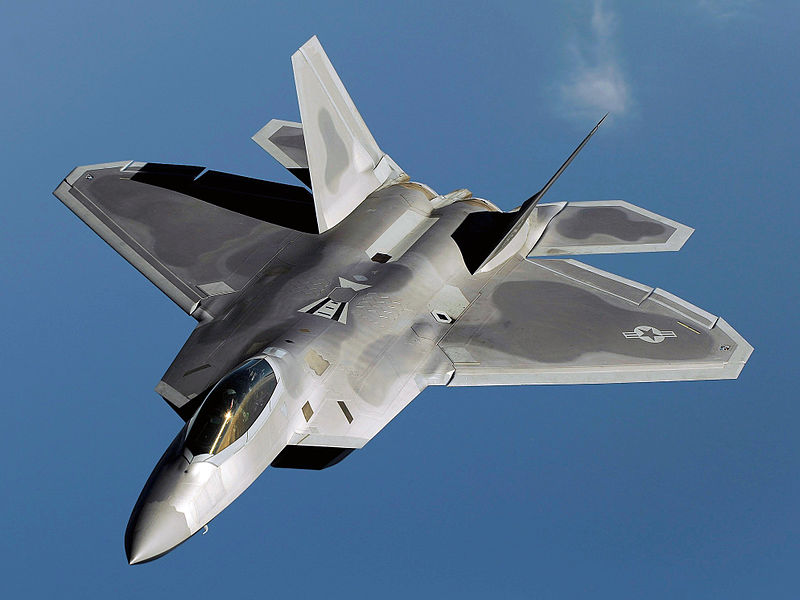
\includegraphics[width=1.75cm]{f22} & F-22 RAPTOR & 38.000 &  2.910 \\
		\pause	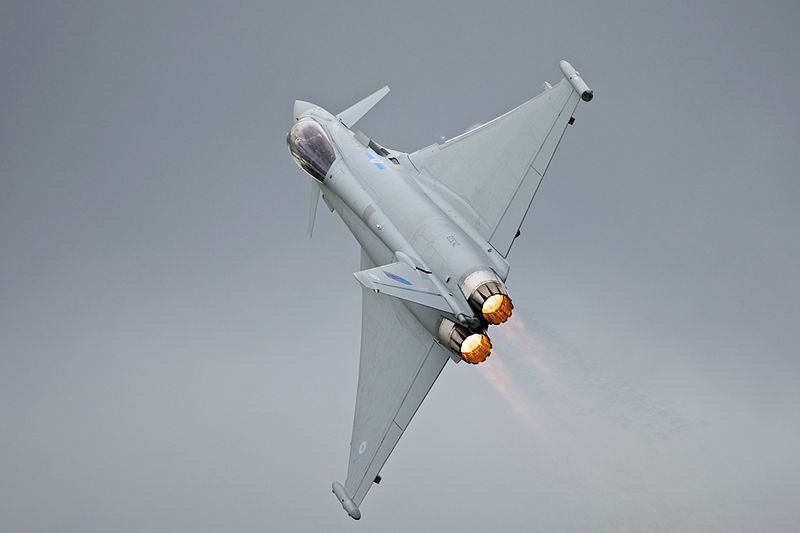
\includegraphics[width=1.75cm]{et} & Eurofighter Typhoon & 23.500 & 2.450 \\
		\pause	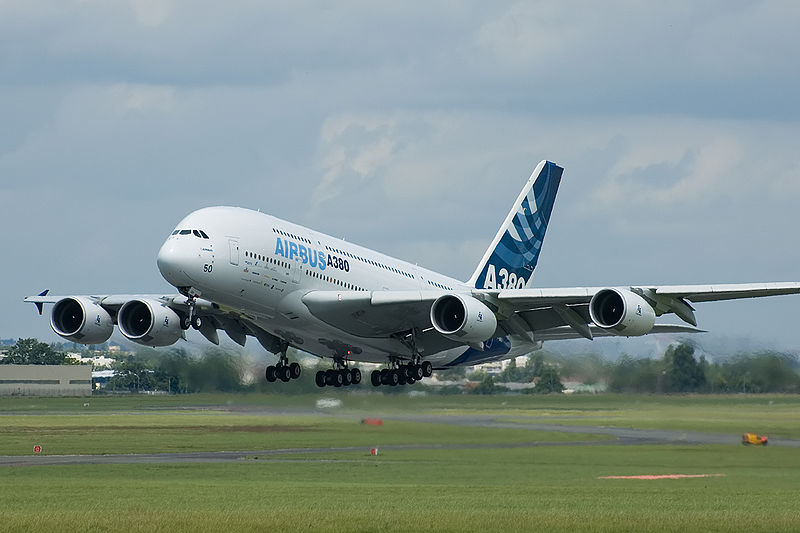
\includegraphics[width=1.75cm]{a380} & Airbus A-380 & 560.000 & 1.100 \\
		\pause	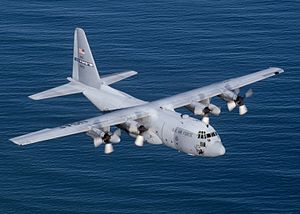
\includegraphics[width=1.75cm]{c130} & C-130 & 71.000 & 592
		\end{tabular}
		\end{center}
		\pause Como puede verse la forma de las alas hace que los aviones se mantengan en el aire independientemente del peso que lleven a una velocidad considerable como he podido mostrar.
	\end{frame}
	 \begin{frame}
	 	\transblindsvertical
	 	\frametitle{Veh�culos terrestres}
	 \pause	La sustentaci�n tiene sentido en los veh�culos terrestres a grandes velocidades. Esto puede encontrarse en los coches de F�rmula 1 o superdeportivos. En este caso los alerones, al contrario con los aviones, hacen que los coches experimentes una fuerza hacia abajo que lo "pega" al suelo. 
	 \pause \par En definitiva la forma de los alerones es la contraria a la forma de las alas de los aviones.
	 \begin{center}
	 	\pause 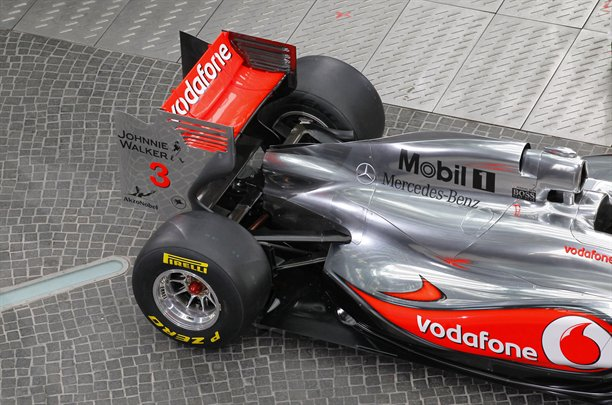
\includegraphics[height=3cm]{aleron1} \hspace{0.5cm}
	 	\pause 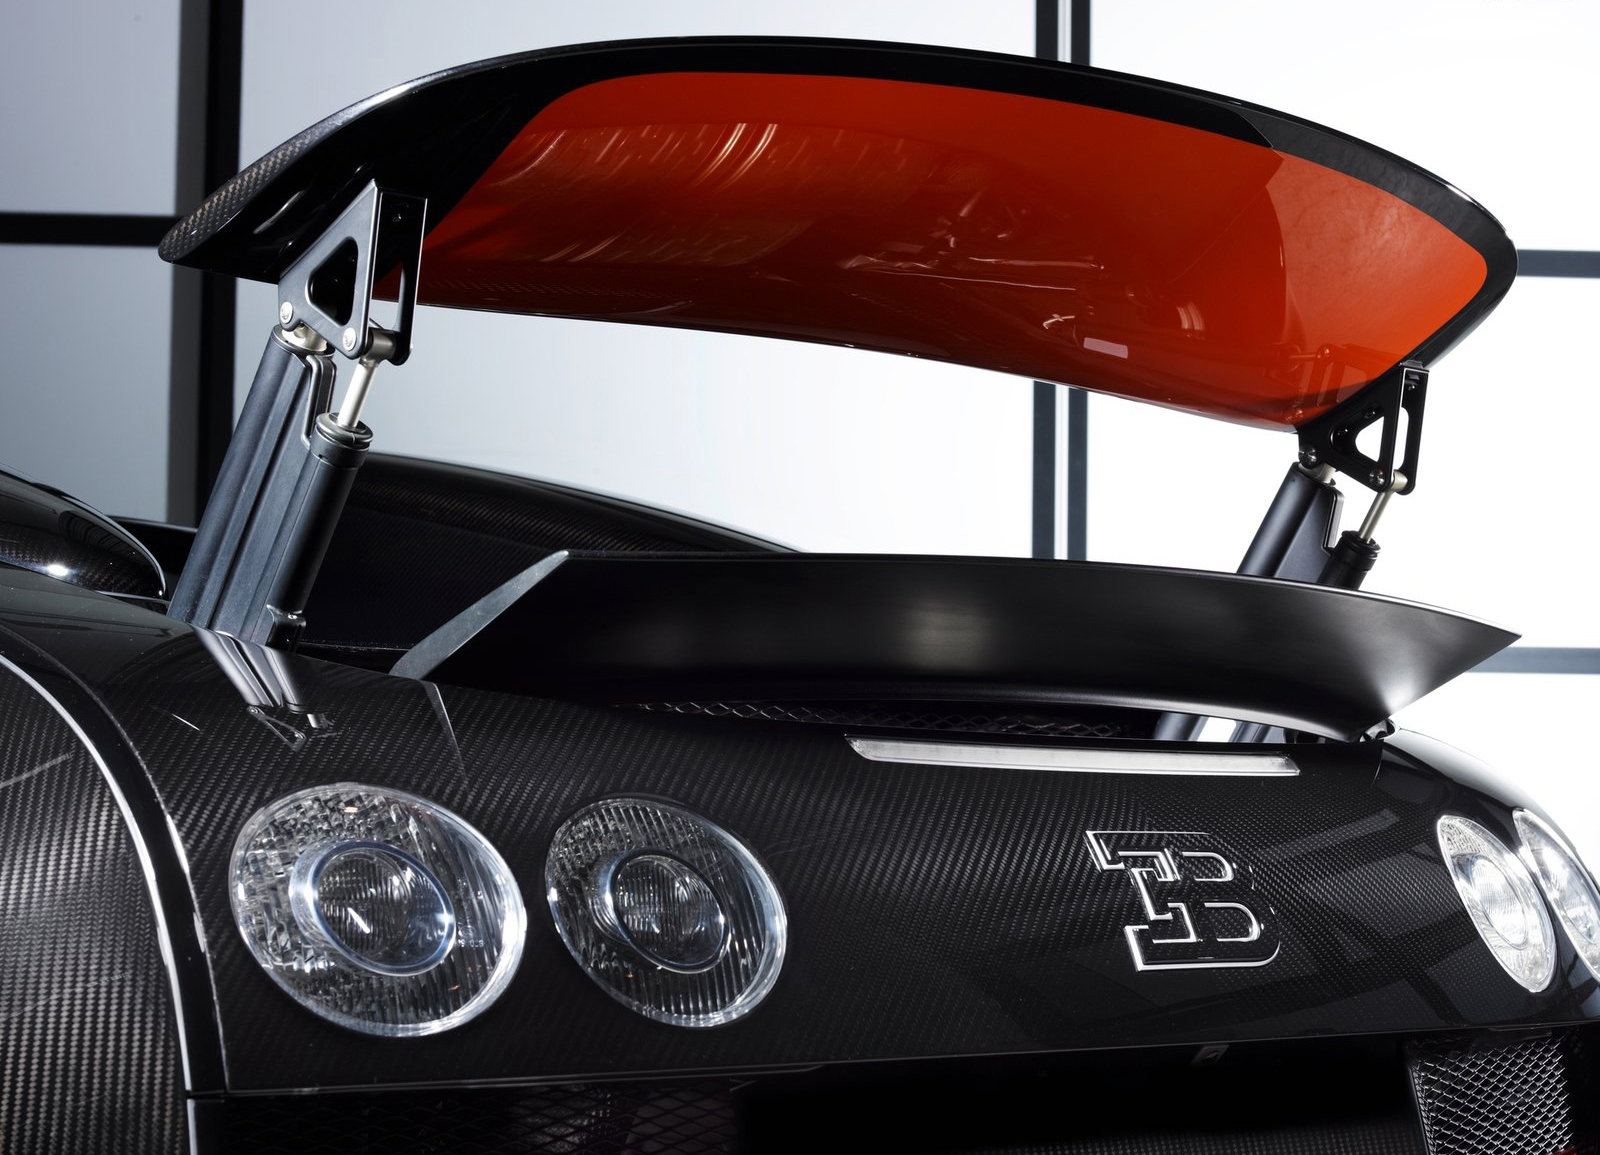
\includegraphics[height=3cm]{aleron2}
	 \end{center}
	 
	 \end{frame}
	
\end{document}